\section{Extraction of CFFs from fits to DVCS observables}\label{sec_michel_fits}

In recent years, various groups have developed and applied different procedures to extract Compton Form Factors from DVCS observables. The approach adopted in this proposal \cite{fitmick,mick_herve} has proved to be very effective and practical to extract GPD information from the existing proton DVCS data\footnote{Eventually, our results will also be compared to the various existing model parametrizations for the GPDs, the free parameters of which will be constrained by our data.}. It is based on a local-fitting method at each given experimental $(Q^2, x_B,-t)$ kinematic point. In this framework, instead of four complex CFFs defined as in Eqs.~\ref{def_cffs1} and \ref{def_cffs2}, there are eight real CFFs-related quantities (which, hereafter will be defined, for brevity, as ``CFFs'')
\begin{equation}
	F_{Re}(\xi,t) = \Re{\rm e}{\cal F}(\xi,t) 
\end{equation}
\begin{equation}
	F_{Im}(\xi,t) = -\frac{1}{\pi}\Im{\rm m}{\cal F}(\xi,t)=\left[ F(\xi,\xi,t)\mp F(-\xi,\xi,t) \right], 
\end{equation}
where the sign convention is the same as for Eq.~\ref{dvcs-ampl}. These CFFs are the almost-free\footnote{The values of the CFFs are allowed to vary within $\pm 5$ times the values predicted by the VGG model \cite{vgg,vgg1}.} parameters, which are extracted from DVCS observables using the well-established DVCS+BH theoretical amplitude. The BH amplitude is calculated exactly while the DVCS one is taken at the QCD leading twist. The expression of these amplitudes can be found, for instance, in \cite{vgg}. 

As there are eight CFF-related unknowns (four ``real'' CFFs, four ``imaginary'' ones) left as free parameters, including more observables, measured at the same kinematic points, will result in more tightly constrained fits and will increase the number and accuracy of CFFs extracted from them. 

This was shown, for instance, with the analysis of the CLAS eg1-DVCS dataset \cite{pisano}, which was taken at 6 GeV with a longitudinally-polarized proton target. The simultaneous fit of three proton-DVCS asymmetries (BSA, TSA and DSA) lead to the extraction of $\Im{\rm m}{\cal H}$ and $\Im{\rm m}{\cal {\widetilde{H}}}$, as is shown in Fig.~\ref{cffs_eg1dvcs}. These results for $H_{Im}$ and ${\tilde{H}}_{Im}$ confirmed what had been previously observed in a qualitative way by direct comparison of the $t$-dependence of the eg1-dvcs TSAs and the e1-dvcs BSAs in \cite{erin}: the $t$-slope of $\Im{\rm m}{\cal H}$ is much steeper than that of $\Im{\rm m}{\tilde{\cal H}}$, hinting at the fact that the axial charge (linked to $\Im{\rm m}{\tilde{\cal H}}$) might be more ``concentrated'' in the center of the nucleon than the electric charge (linked to $\Im{\rm m}{\cal H}$). This is an interesting example of the nucleon tomography that becomes possible with the determination of CFFs, without the need for model input. 

The main goal of the experiment proposed here is to provide, in a wide phase space, two kinds of asymmetries (single-target, and double beam-target), to be simultaneously fitted together with the beam-spin asymmetry that will be measured, at the same kinematic points, in the approved unpolarized-target experiment \cite{proposal}, and thus allow the extraction of the neutron CFFs. The results we expect to obtain are presented in Section \ref{sec_cff}. 

\begin{figure}[tbph]
\begin{center}
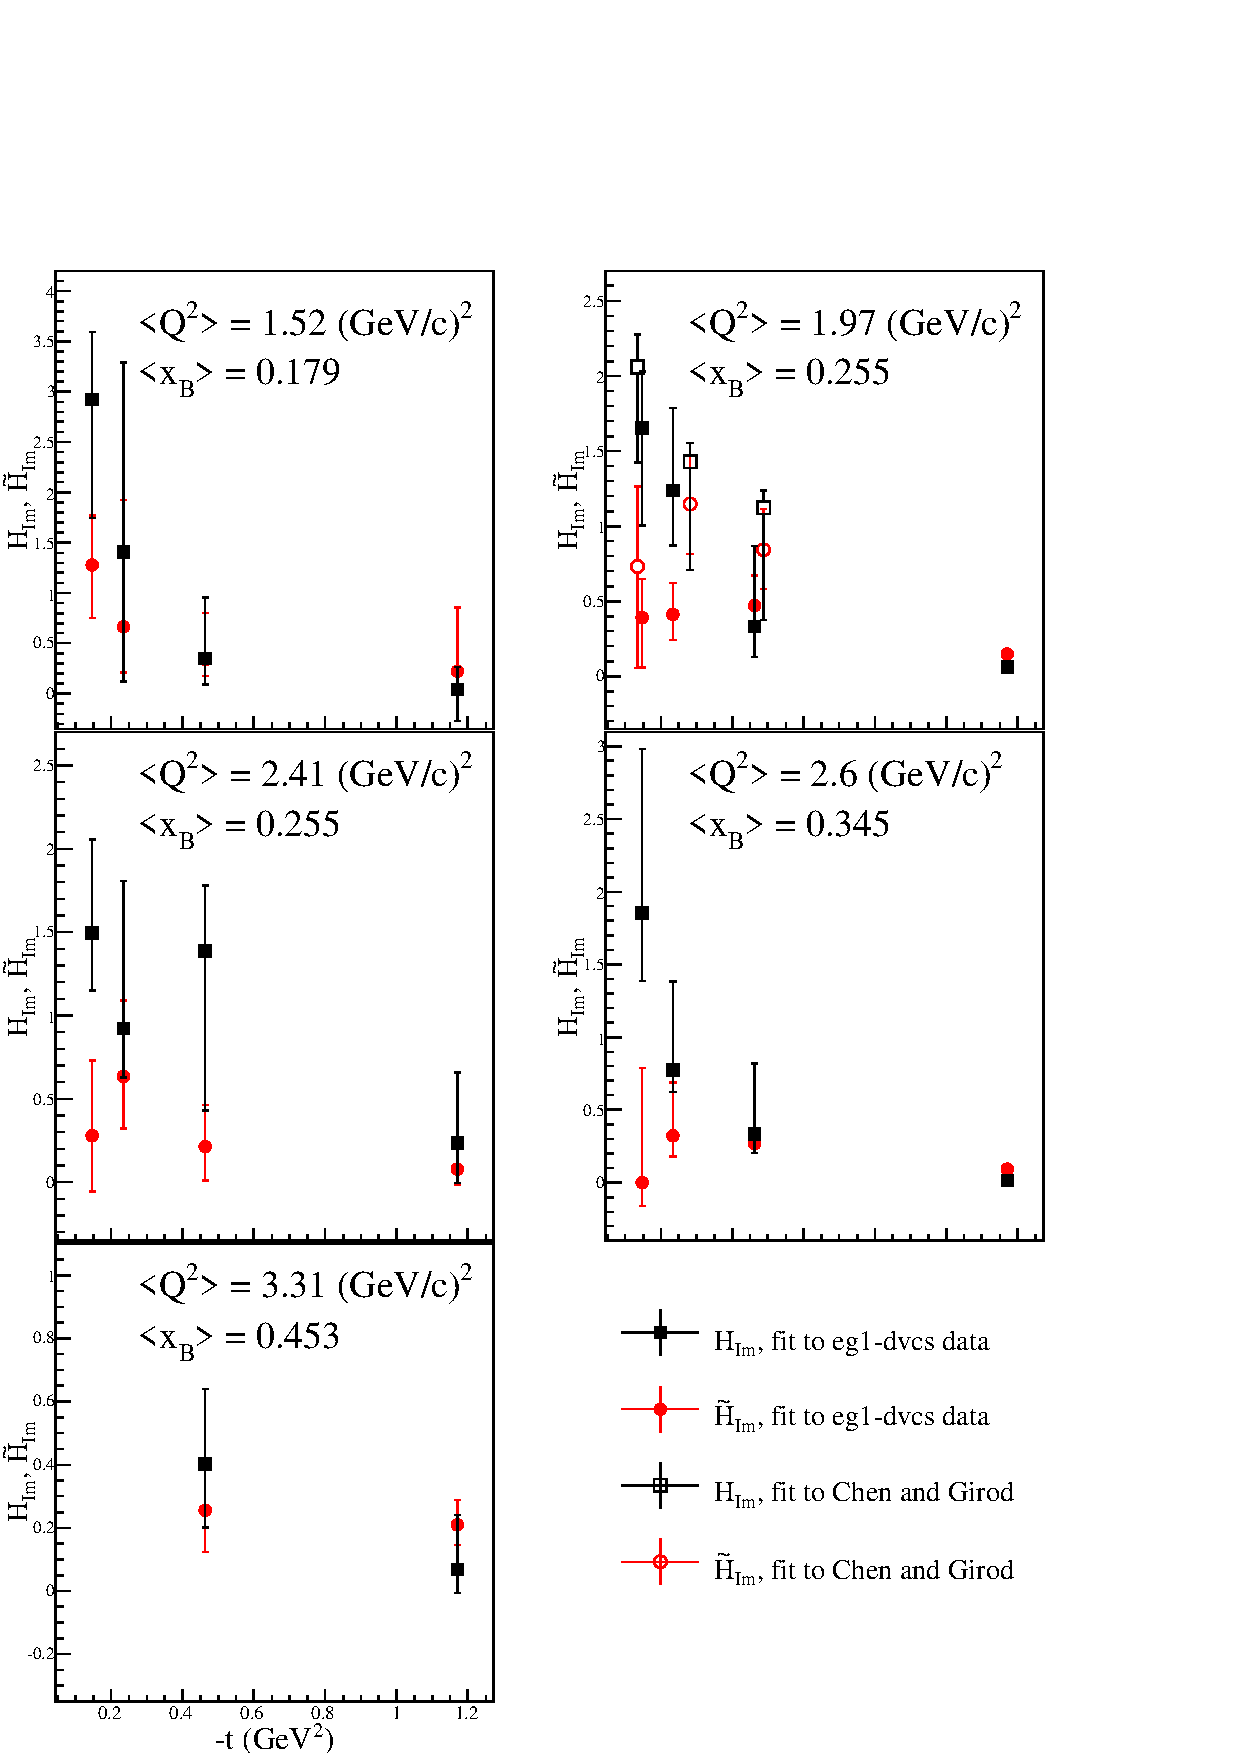
\includegraphics[width=120mm]{CFF_comp_prop.pdf}
\caption[$t$ dependence of $H_{lm}$ and $\tilde{H}_{lm}$.]
{$t$ dependence for each $Q^2$-$x_B$ bin of $H_{Im}$ (black squares) and $\tilde{H}_{Im}$ (red circles). The full points are obtained by fitting the eg1-DVCS data (TSA, BSA and DSA) \cite{pisano}. The empty points were obtained by fitting the BSA results from \cite{fx} integrated over all values of $Q^2$ at $x_B \sim 0.25$, and the TSAs from \cite{shifeng}.}
\label{cffs_eg1dvcs}
\end{center}
\end{figure}
